\chapter{Theoretische Grundlagen}
%\addcontentsline{toc}{chapter}{Grundlagen}
\section{Der Cubesat Designstandard}
	\subsection{Historische Entwicklung}
Die Fortschritte in der modernen Technologie unterstützen die Entwicklung der miniaturisierten Satelliten. Durch den Fokus der wissenschaftlichen Gemeinschaft auf Nano- und Picosatelliten sind die CubeSats zu einem wichtigen Teil der Kategorie geworden. Mit der Einführung des CubeSat-Konzepts 1998, mit der die Standardisierung von Masse und Größe von Satelliten inher ging, stieg die Zugänglichkeit des Weltraumes \cite{RahmatSamii.2017}. Des Weiteren zeichnen sie sich durch ihre Modularität, leistungsstarken und kommerziell erhältlichen Satellitenkomponenten (commercial off-the-shelf) und ihren schnellen Entwicklungszyklen aus \citavi{}. Infolge der Standardisierung des CubeSats wurde das Startsystem Poly-Picosatellit Orbit Deployer (P-POD) entwickelt um eine kostengünstige Lösung für die Entwicklung und den sicheren Start bereitzustellen \cite{RahmatSamii.2017}. 2003 wurde die  erste CubeSat Mission durchgeführt. Seitdem werden sie mit stark zunehmender Häufigkeit eingesetzt. Dies wird in \abb{fig:NanosatsTypes} veranschaulicht.
			\begin{figure}[h]
				\centering
					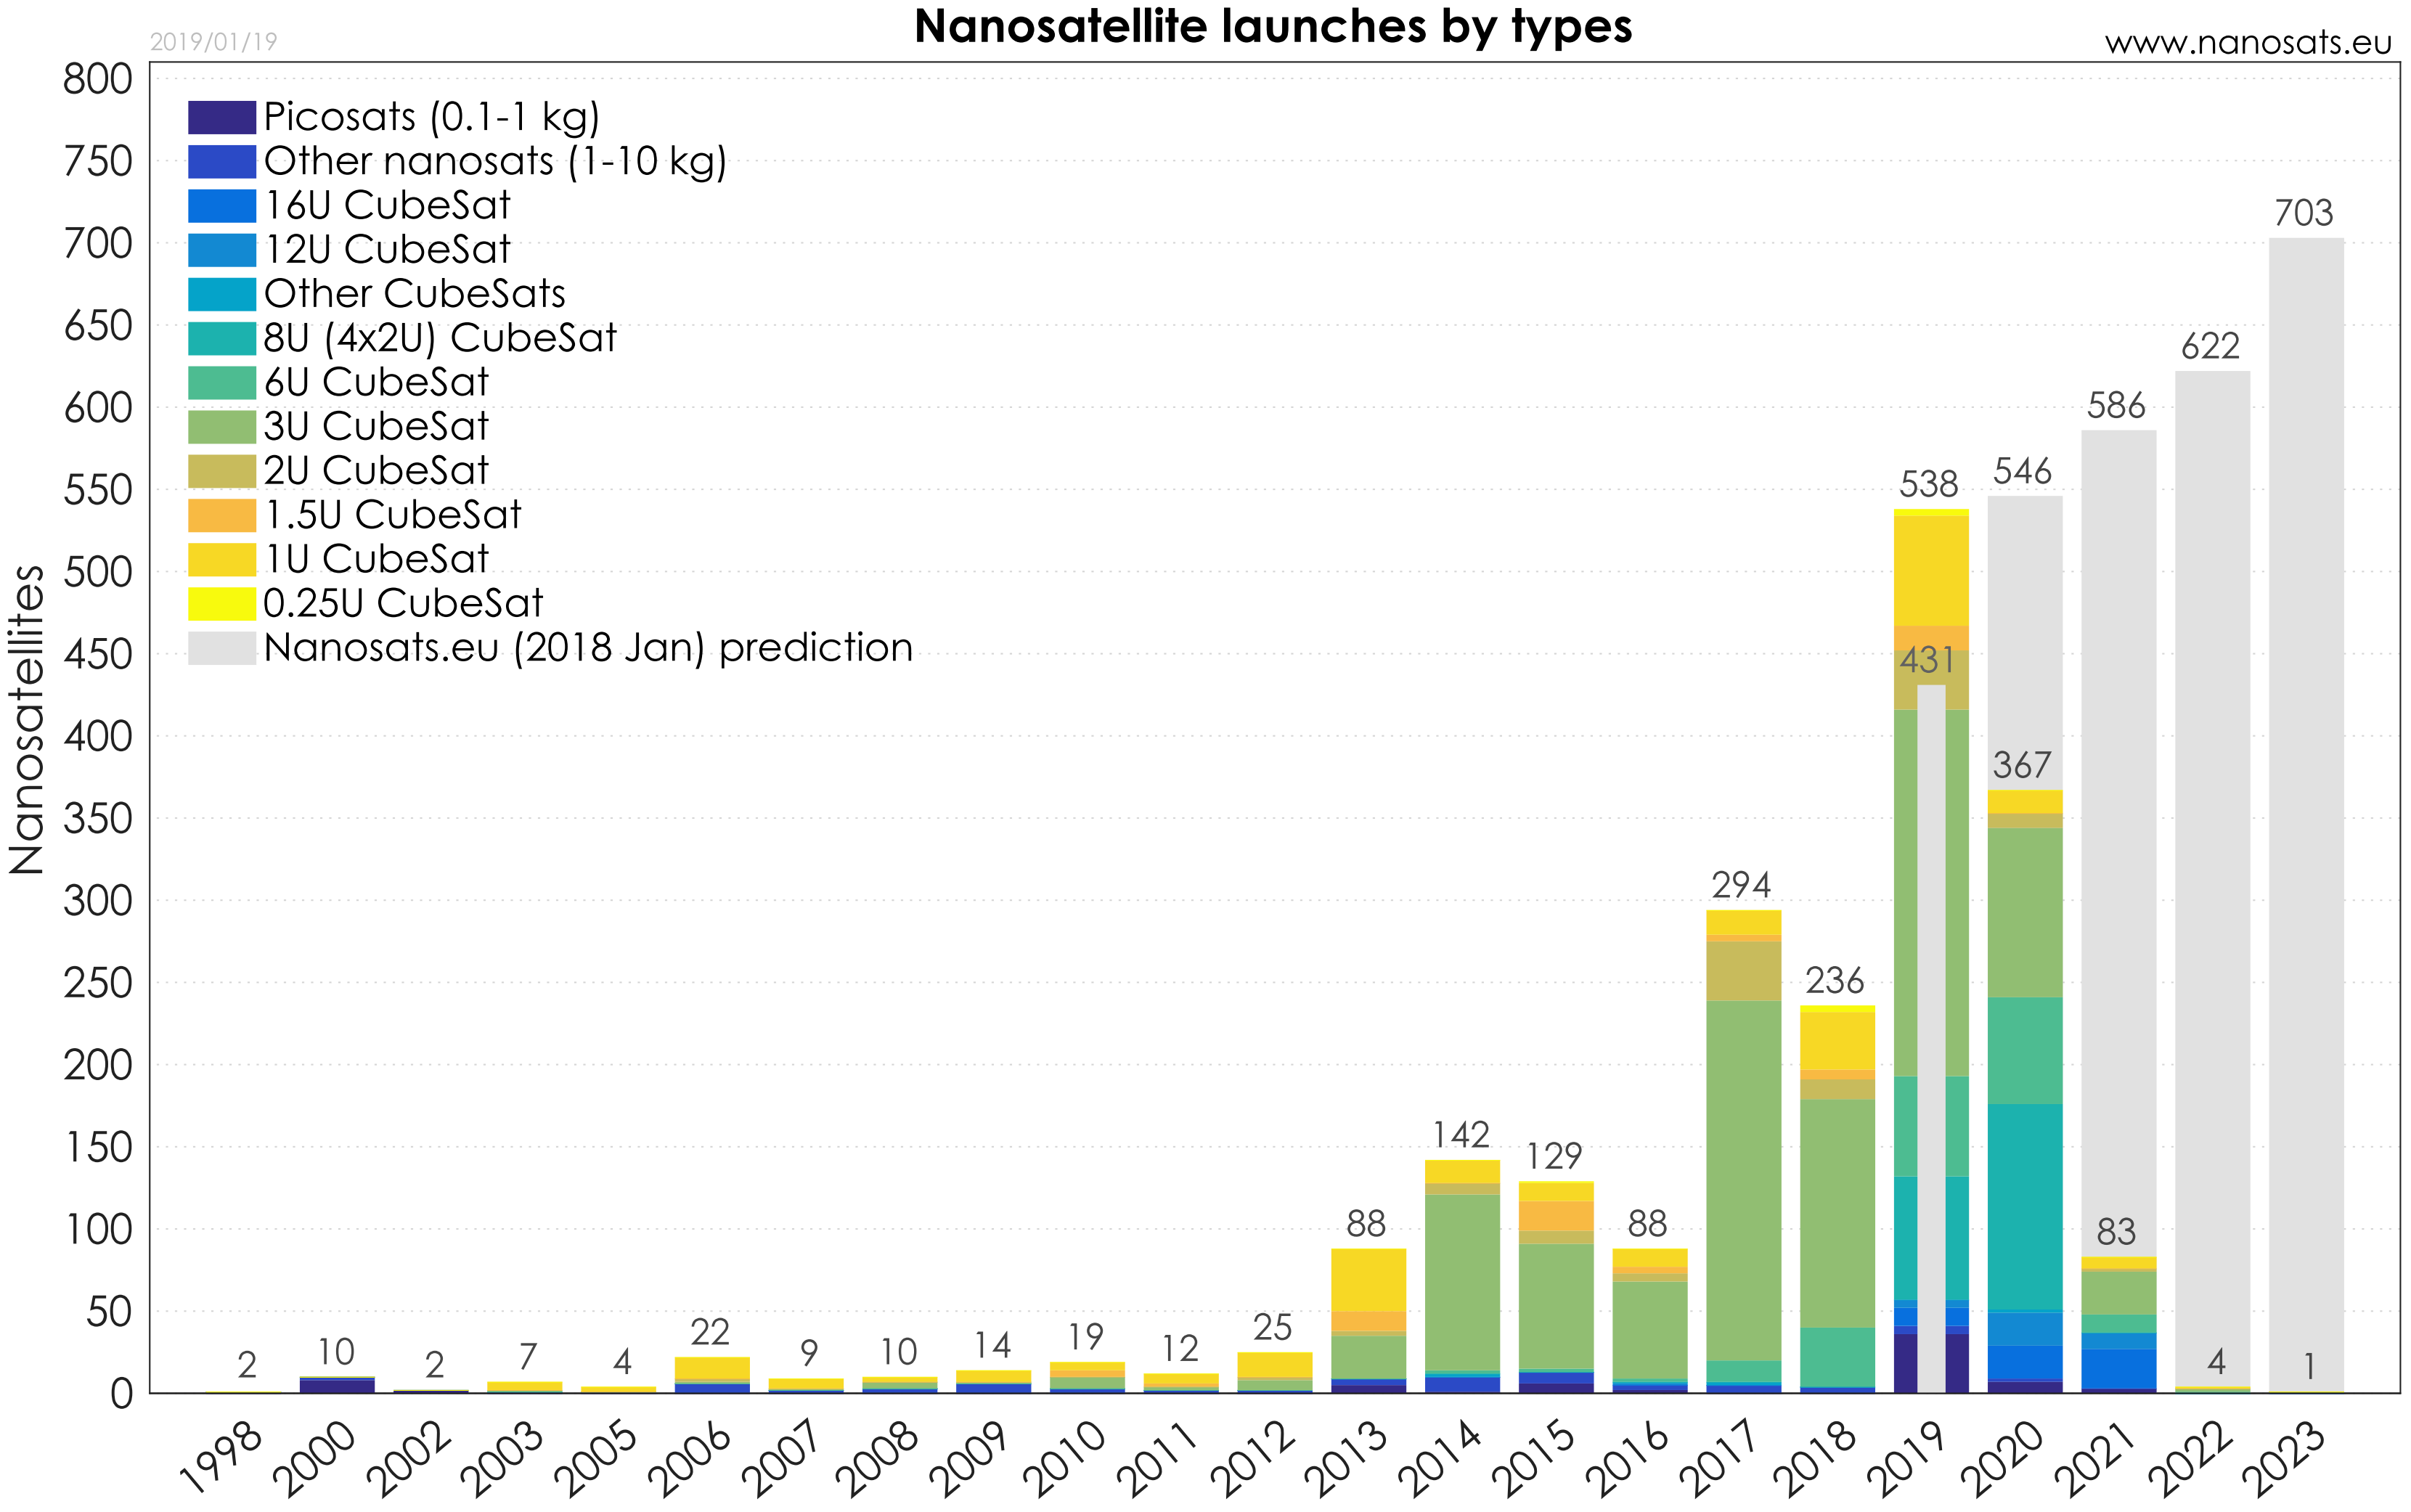
\includegraphics[width=0.80\textwidth]{Nanosats_years_types_2019-01-19_01}
				\caption{Überblick über Nanosatelliten.Missionen von 1998 bis 2023}
				\label{fig:NanosatsTypes}
			\end{figure}

	\newpage
	\subsection{Gestaltungsrichtlinien}
		
	\begin{-}
Für die Gestaltung von CubeSats gelten eine Reihe von Richtlinien. Als kleinste Einheit (1U) wird ein Würfel mit einer Kantenlänge von 10cm und einer zulässigen Masse von maximal 1,33 kg vorgegeben. Für größere Volumen und Massen können mehrere Einheiten von CubeSats verbunden werden. Satelliten mit 1U, 1.5U, 2U, oder 3U können von dem einheitlichen Startmechanismus (P-Pod) in die Erdumlaufbahn ausgelassen werden. Die Kosten von CubeSat Missionen können gering gehalten werden, indem diese als sekundäre Nutzlast bei Raketenstarts mitfliegen. Für größere Satelliten (6U, 12U, 27U) werden andere Startmechanismen benötigt. Die zugelassene Masse wird auf 2 kg/U angehoben. Weitere Vorschriften gelten für die Folgenden Kriterien:
		\begin{itemize}
			\item \textit{Materialien:} 	\\ Alle bei der Konstruktion verwendeten Materialien müssen den Richtlinien der Air Force Space Command Manual \textbf{[AFSPCMAN 91-710 Volume 3]} entsprechen. Außerdem darf der Masseverlust des Satelliten maximal 1\% betragen.
			\item \textit{Energiespeicher:} \\ Der chemische Energiespeicher darf eine Größe von 100 Wh nicht überschreiten. 
			\item \textit{Aktivierungszeitpunkt:} \\ Während der CubeSat im P-POD verstaut ist müssen alle Systeme ausgeschaltet bleiben. Beim Verlassen der Trägerrakete wird der Satellit aktiviert. Erst 30 Minuten später dürfen Bauteile (z.B. Solarpanele, Antennen, etc...) ausgefahren werden. Bevor die ersten Signale generiert oder gesendet werden müssen mindestens 45 Minuten vergangen sein. 
		\end{itemize}
%Allgemein gelten noch weitere Vorschriften für die verwendeten  Materialien, Kommunikationsfähigkeit, gespeicherte Energie und Aktivierungszeitpunkt der Systeme nach Einsatz in die Umlaufbahn. 
Falls ein Entwurf nicht den Vorschriften entspricht, kann bei dem Betreiber der Trägerrakete eine Sondergenehmigung angefragt werden. Nach einer Reihe von Tests entscheidet dieser ob er die Abweichungen akzeptiert, Änderungen vorgenommen werden müssen, oder ein anderer Anbieter gefunden werden muss. 
		\end{-}

			
	\section{Cubesat Subsysteme}
	hier Hauptsächlich das Fazit von max kompakt darstellen und refernzieren
		\subsection{Antrieb - propulsion}
		\subsection{Energie - EPS}
		\subsection{Guidance, navigation and control -GNC ADCS}
		\subsection{Command and data handling}
		\subsection{Communications}
		\subsection{Thermal}
		\subsection{Structure}
				
	\section{RDVDO Mechanismen} das kann ausführlich sein
		\subsection{Docking Strategien}
						\textbf{Roboterarm}
						\textbf{Fangnetz}
						\textbf{Adhäsiv Docken}
						Übersichtstabelle/Graphik: sihe die Quellen die ich am 15.05.2019 gezeigt habe
		\subsection{Bionische Materialien}
						\textbf{Was sind Geckomaterialen}
						\textbf{Bisher getestete Gecko-Materialien}
						\textbf{Bisherige Erfolge}
						\textbf{State of the Art}
						\textbf{Problematik}